\documentclass[nogrid]{MBE}%


\usepackage{url}

\usepackage{lineno}
\linenumbers

\jshort{mst}

\volname{}

\jvolume{0}

\jvol{}

\jissue{0}

\pubyear{2017}

\mstype{Article}

\artid{}

\access{}


\begin{document}

\title[Constrained ordination for environmental genomics]{Constrained ordination method as a tool for performing genome scan and environmental genomic studies}


\author[Bazin et al.]{Eric \surname{Bazin},$^{\ast,1}$ Keurcien Luu,$^{2}$ Michael G. B.
Blum,$^{2}$}

\address{$^{1}$LECA, Universit\'{e} de Grenoble\\
$^{2}$TIMC, Universit\'{e} de Grenoble}


\history{}

\coresp{E-mail: eric.bazin@univ-grenoble-alpes.fr}

\datade{}


\editor{}

\abstract{
}

\keyword{}

\maketitle



\section{{Introduction}\label{sec:Intro}}


Performing genome scan in order to detect genomic region of interest is a common task in population genomic area \citep{Foll2008,Frichot2013,Luu2016,Vatsiou2015}. Some methods aim at detecting  genes that has suffered from a loss of genetic diversity and increase of linkage disequilibrium following the appearance of a beneficial allele and its spread by the mean of selective sweep. Others aim at picking up alleles with strong correlation with some environnemantal variable (e.g. Temperature, drought) with the idea that these alleles may confer a selective advantage to the individuals  \citep{Coop2010,Frichot2013}. Finally, other methods aim at detecting genomic region involved in local adaptation process. These region should have an increased differentiation between population because different alleles tend to be beneficial in each environment. Differentiation between population is excepted under the hypothesis of geographical isolation. Therefore, this region can be detected by quantifying the level of differentiation using some statistics and detecting the regions with unexpectedly high values. A common statistic and very easily comprehensible in population genetic is Fst. Many methods use this parameter as a basis in many different implementation of genome scans \citep{Bazin2010,DeVillemereuil2015,Foll2008}. These are model based method where parameters such as Fst are usually inferred using likelihood or Bayesian methods. This mean that users must have some a priori on their parameter value and the best model that fits their data in order to expect the best from their analysis.
	However, it is often difficult to get a satisfactory a priori picture of the demographic and population structure of the species one is interested in. Indeed many species are not clearly structured in different populations but more or less show a pattern of isolation by distance without clear geographical barrier to gene flow. One solution would be to use more complex model that better reflect reality but these are difficult to implement in Bayesian framework. Additionally, these latter methods are very time consuming and the increase of both model complexity and the amount of data to analyze in terms of the number of individuals and loci makes them more and more difficult to use.
	A new path has opened recently with the use of multivariate methods. The idea is to capture the whole genome geographic structure using an ordination method such as ACP. Following this analysis, outliers loci are detected if they have extremely high correlation with one or more ordination axis \citep{Duforet-Frebourg2014a,Luu2016}.  These are very efficient methods and simulations have shown that while they are very fast, they show similar efficiency than classical Bayesian method and sometimes perform better when the simulated demographic model drift from the model implemented in bayesian method, usually the island model. For instance \citet{Luu2016} have shown their method to be better when population are structured in hierarchical set or in isolation by distance pattern. Nevertheless, one conundrum of such approaches is the difficulty to interpret ordination axis in term of ecological meanings. These are usually tight to geographical axis (latitudinal or longitudinal) but they are not necessary linked to an environmental variable such as Temperature, drought, diet habit, etc. Therefore, when this information exists, it has to be a posteriori used as a mean of interpretation but are not involved in the inference process.
	It should be recalled that natural selection is the result of a complex set of environmental pressures and that it most often acts on several characters simultaneously and that these characters are encoded by several genes which generally have weak effects. In order to extract the maximum of all available information, it seems therefore necessary to use approaches that are able to compile all kind of variable (e.g. alleles, phenotypic measurement, biotic and abiotic variables).
	One natural way to overcome this limitation would be to use more sophisticated ordination method than ACP like methods. Constrained ordination methods (i.e. Redundancy Analysis, RDA, Canonical Correspondence Analyis, CCA) are well-known set of approaches in Ecology for instance to explain the species distribution pattern by the mean of environmental data. They have specifically been designed in order to deal with biological complexity. In the population genomic era, it seems that data amount, complexity and heterogeneity is often a limitation to the use of inference methods based on classical population genetic models. Although they are more difficult to interpret, such approaches would be complementary to the model based method because of their long-term use in ecology and their efficiency on complex and large datasets. These method have sometimes been used in population genomic studies, not as a genome scan but in order to quantify multilocus adaptation to an environmental gradient \citep{Lasky2012,DeKort2014,Steane2014a,Hecht2015}. These studies whereby relationships between environmental data and large multilocus data is explored are becoming more and more popular and are often coined as Ecological Genomics or Landscape Genomics studies. However the concept of using constrained ordination methods to analyse genomic data has never been tested on simulated datasets.
	This paper aims at filling this gap. First, we show how one can make use of a constrained ordination method namely Redundancy Analysis (RDA) as an efficient and robust genome scan method. We discarded the other constraint ordination methods such as CCA since they are very similar in their principles. RDA has already been used for instance by \citet{Lasky2012} to perform genome scan in order to detect loci involved in the adaptation to climate in \textit{Arabidopsis thaliana}. Outliers were identified as SNPs with the greatest squared scores along the first RDA axis (i.e. those in the 0.5 \% tail). We build on this idea to develop a comprehensive and robust statistical test that allows to search for outliers on an arbitrary number of RDA axis simultaneously and allows to control precisely for the false discovery rate. Using simulations, we show that it has better results than PCA-based method. Second, thanks to these simulations, we show that RDA can indeed help to identify important environmental gradient that better explain the adaptive variation in the data. It is therefore a proof of concept of the idea of using constrained ordination method as an environmental genomic tool to identify relevent selective gradient in the environmental data. Finally, to give a concrete illustration of RDA approach in population genomics, we apply this method to the detection of outliers on a real data set.

\section{Material and method}

\subsection{Genome scan}

Redundancy analysis (RDA) was first introduced by \citep{Rao1964} and is clearly described in \citep{Legendre2012} section 11.1. It is the direct extension of multiple regression to the modeling of multivariate response data. Typically the data to be analysed are separated in two sets, a response matrix Y of variable to be explained (e.g. species abundance in a set of sites; m sites and n species) and an explanatory matrix X (e.g.  a set of environmental variable within each site; m sites and p environment). 
	In the following analysis, species are replaced by loci and sites by individuals. In other word, we wish to project on a reduced space the proportion of variance in genetic difference between individuals which is better explained by environmental data.
	After this ordination, we follow the \citet{Luu2016} methodology to compute pvalues. First we compute the test statistic by regressing each of the p SNPs by the K ordination axis $X_1, ..., X_K$.

$G_j = \sum^{K}_{k=1}\beta_{jk}X_{k}+\epsilon_{j}, j=1,...,p$

where $\beta_{jk}$ is the regression coefficient corresponding to the j-th SNP regressed by the k-th ordination axis, and $\epsilon_{j}$ is the residuals vector. To summarize the result of the regression analysis for the j-th SNP, we return a vector of z-scores $z_{j} = (z_{j1}, ..., z_{jK})$ where $z_{jk}$ corresponds to the z-score obtained when regressing the j-th SNP by the k-th ordination axis.
The test statistic is a robust Mahalanobis distance D computed using covRob function of the robustR package. D should be Khi2 distributed after a correction with inflation factor (Luu et al., 2016). Pvalues are computed using K degree of freedom. We use the FDR approach to control for false positives. Qvalue are computed with qvalueR package and a loci is considered as an outlier if its qvalue is less than 10\%.
For the analysis of simulated dataset (see below), we retain the first four ordination axis to compute Mahalanobis distances  as they seem to explain most of the variance in the data. To peform the ordination, we use the 10th environmental variables as input in the explanatory matrix. In the following example, we don't use phenotypic informations since these informations are often laking in environmental genomics. Neither we use geographical coordinates $(i,j)$ which is sometimes added to control for the geographical covariation in the differentiation pattern \citep{Frichot2013}.

To emphasize the utility of RDA, we compared to pcadapt from which the idea of using multivariate method for genome scan is based. On the simulated dataset, we retain $K=3$ axis to compute Mahalanobis distances  as it seems to explain the main amount of variance in the data using scatter plots. To control for false positive, we used the same qvalue threshold (i.e. <= 10\%).


\subsection{Environmental genomic}

Once outliers have been identified, we isolate them in a separate matrix A defining an "adaptively enriched genetic space" as coined by \citet{Steane2014a}. Following their methodology, we perform a second constrained ordination (RDA) on matrix A against environmental data. The rational of this analysis is to remove neutral variation before performing ordination in order to have a better picture of which environmental gradients have the strongest association with the adaptive genetic space. On the simulated dataset, we report the $R^2$ statistics between env1, env2 and env3 and the first three ordination axis to have an idea of which they are better associated with and if the ordination space succeed in seperating the environmental effect on different axis.


\subsection{Simulations}

To test for the efficiency of RDA in population genomic, we performed simulations using simuPop python library \citep{Peng2005}. We compared our approach to PCAdapt method to perform genome scans. Both approach are equivalent except their ordination method. Finally we use these simulations to evaluate RDA approach as a mean to detect selective environmental gradient.
	A lattice of 8x8 populations is simulated (i.e. 64 populations in total). Each population is initialized with 200 diploid individual with random genotypes. Migration is set to 0.5 so that population structure must be very smooth and genetic differentiation must show an isolation by distance pattern over the 64 populations. This is where pcadapt is best designed for. Loci are biallelic (0 or 1) like SNPs. Allele frequency of the whole population is initialized at 0.5. 1000 loci are defined. They are separated in 200 chuncks of 5 SNPs in physical linkage with recombination rate between adjacent loci fixed at 0.1. 3 different Traits are coded by a group of 10 different loci. The first trait is coded by loci 1, 11, 21, ..., 91. The trait value is simply the sum of genotype value and therefore can take value between 0 an 20. For the sake of realism, we add to each trait a random noise (non heritable variation) drawn from a normal distribution $N(0,2)$. The second trait is coded by loci 101, 111, ..., 191 and the third is coded by loci 201, 211, ..., 291. Each trait is therefore coded by free recombining SNP loci. In other words, there are 30 coding SNPs among 1000. Selection can have an effect on linked loci, for instance, loci 2, 3, 4 and 5 can be impacted by selection on locus 1. However, recombination is high enough (0.1) to expect a limited linkage effect. We have defined 10 different environmental variables. The first one determines the selective pressure on trait 1, the second one on trait 2 and the third one on trait 3. The first environment variable is a quadratic gradient coded by function  $env1 = -(\cos(\theta)*(i-3.5))^2 -(sin(\theta)*(j-3.5))^2 + 18, \theta = \pi/2$, i and j being the population indicator on the 8x8 lattice. The second one is a linear plan gradient coded by function $env2 = h*\cos(\theta)*(i-1) + h*\sin(\theta)*(j-1) + k$ with $h=2$, $\theta = \pi/4$ and $k=3$. The third environment variable simulates a coarse environment with value $env3 = 2$ for all populations except population (i,j) = {(2,2), (2,3), (3,2), (3,3), (6,2), (6,3), (7,2), (7,3), (2,6), (2,7), (3,6), (3,7), (6,6), (6,7), (7,6), (7,7)} for which $env3 = 18$. Env4, env5 and env6 have exactly the same equation than env1, env2 and env3 respectively. The remaining 4 environment variable are similar to env2 but with different value of h and $\theta$. Env7 has $h=2$, $\theta = 0$ and $k=3$. Env8 has $h=2$, $\theta = \pi/4$ and $k=0$. Env9 has $h=1$, $\theta = \pi/4$ and $k=4$. Env10 has $h=0.5$, $\theta = \pi/4$ and $k=8$. Graphical representation of mean environmental value for environment 1, 2 and 3 is given in Fig. \ref{simulatedenvir}. Environment 4, 5 and 6 have respectively the same mean value spatial distribution. For a graphical representation of environment 7 to 10, see supplementary material. Environmental equation gives a mean value of the environment variable. To avoid colinearity between environments variable, we added noise by drawing an environment value within a normal distribution $N(\mu=env, \sigma=1)$. Fitness for each trait is set to be $-e^{((x-env)^2/(2*\omega^2))}$, $x$ being the quantitative trait value, $env$ the environmental value and $\omega$ is defining selection strength and has been set to 10 which in our experience seems sufficient for loci to be often detected. To get the overall fitness for a given individual, fitness associated to each trait are multiplied. Fitness are relative and selection arises on parents and determine their number of offsprings. Simulations are made across 500 generations. At the end of simulation, we sample 10 individuals per population. Therefore, we have a sample of 640 individuals with 1000 SNP-like loci.

\subsection{Real dataset}
The Loblolly pine dataset is a sample of 682 individuals genotyped on 1,730 SNPs selected in ESTs \citep{Eckert2010}. 60 climatic variables were available and summarized by the authors in the five first axis of a PCA. The first axis, PC1 is mainly linked to latitude, longitude, temperature, and winter aridity. PC2 is linked to longitude, spring-fall aridity, and precipitation. We inputed the missing data using a very simple algorithm implement in function sing.im of the R package linkim \citep{Lachenbruch2011}. It imputes the missing value based on the observed data proportions.  We used $K=4$ axis to compute Malahanobis distances.

The Chinook salmon consists of 19 703 SNP loci genotyped on 1956 total individuals pooled in 46 collections. Five variables (MigDistKM, StreamOrder, bio03, bio17 and bio18) have been used among  24 different climate and environmental variables because they have been tested as significantly associated with the SNP variation rangewide citep{Hecht2015}. MigDistKM stands for Migration distance from collection site to ocean (km),
StreamOrder for Stream Order of collection site using Strahler method, bio03 for Isothermality, bio17 for Precipitation of Driest Quarter (mm) and bio18 for Precipitation of Warmest Quarter (mm). We could have tested more variable but this is just an illustration and is by no mean an extensive study of this species. Since data are pooled, we have randomly created a sample of 100 individuals for each collection based on the allele frequencies to be able to analyze the data following our individual based pipeline. We used $K=4$ axis to compute Malahanobis distances.


\section{Results}

\subsection{Genome scan}

When looking at the analysis on one simulation, the pcadapt method seems successful at detecting QTL2 SNPs (Fig. \ref{fig:pcadapt}) but fails at detecting QTL1 and QTL3 SNPs. On the other hand, RDA succeeds at detecting QTL2 SNPs and also some of the QTL1 and QTL2 SNPs (Fig. \ref{fig:rda}). The ordination seems to correctly detect environmental variable 1 and 3 as drivers of genetical variance in the data. Over the 100 simulations, we have measured the average FDR and power for both pcadapt and RDA (Fig \ref{fig:performance}). 


\begin{figure*}[t]
\begin{center}
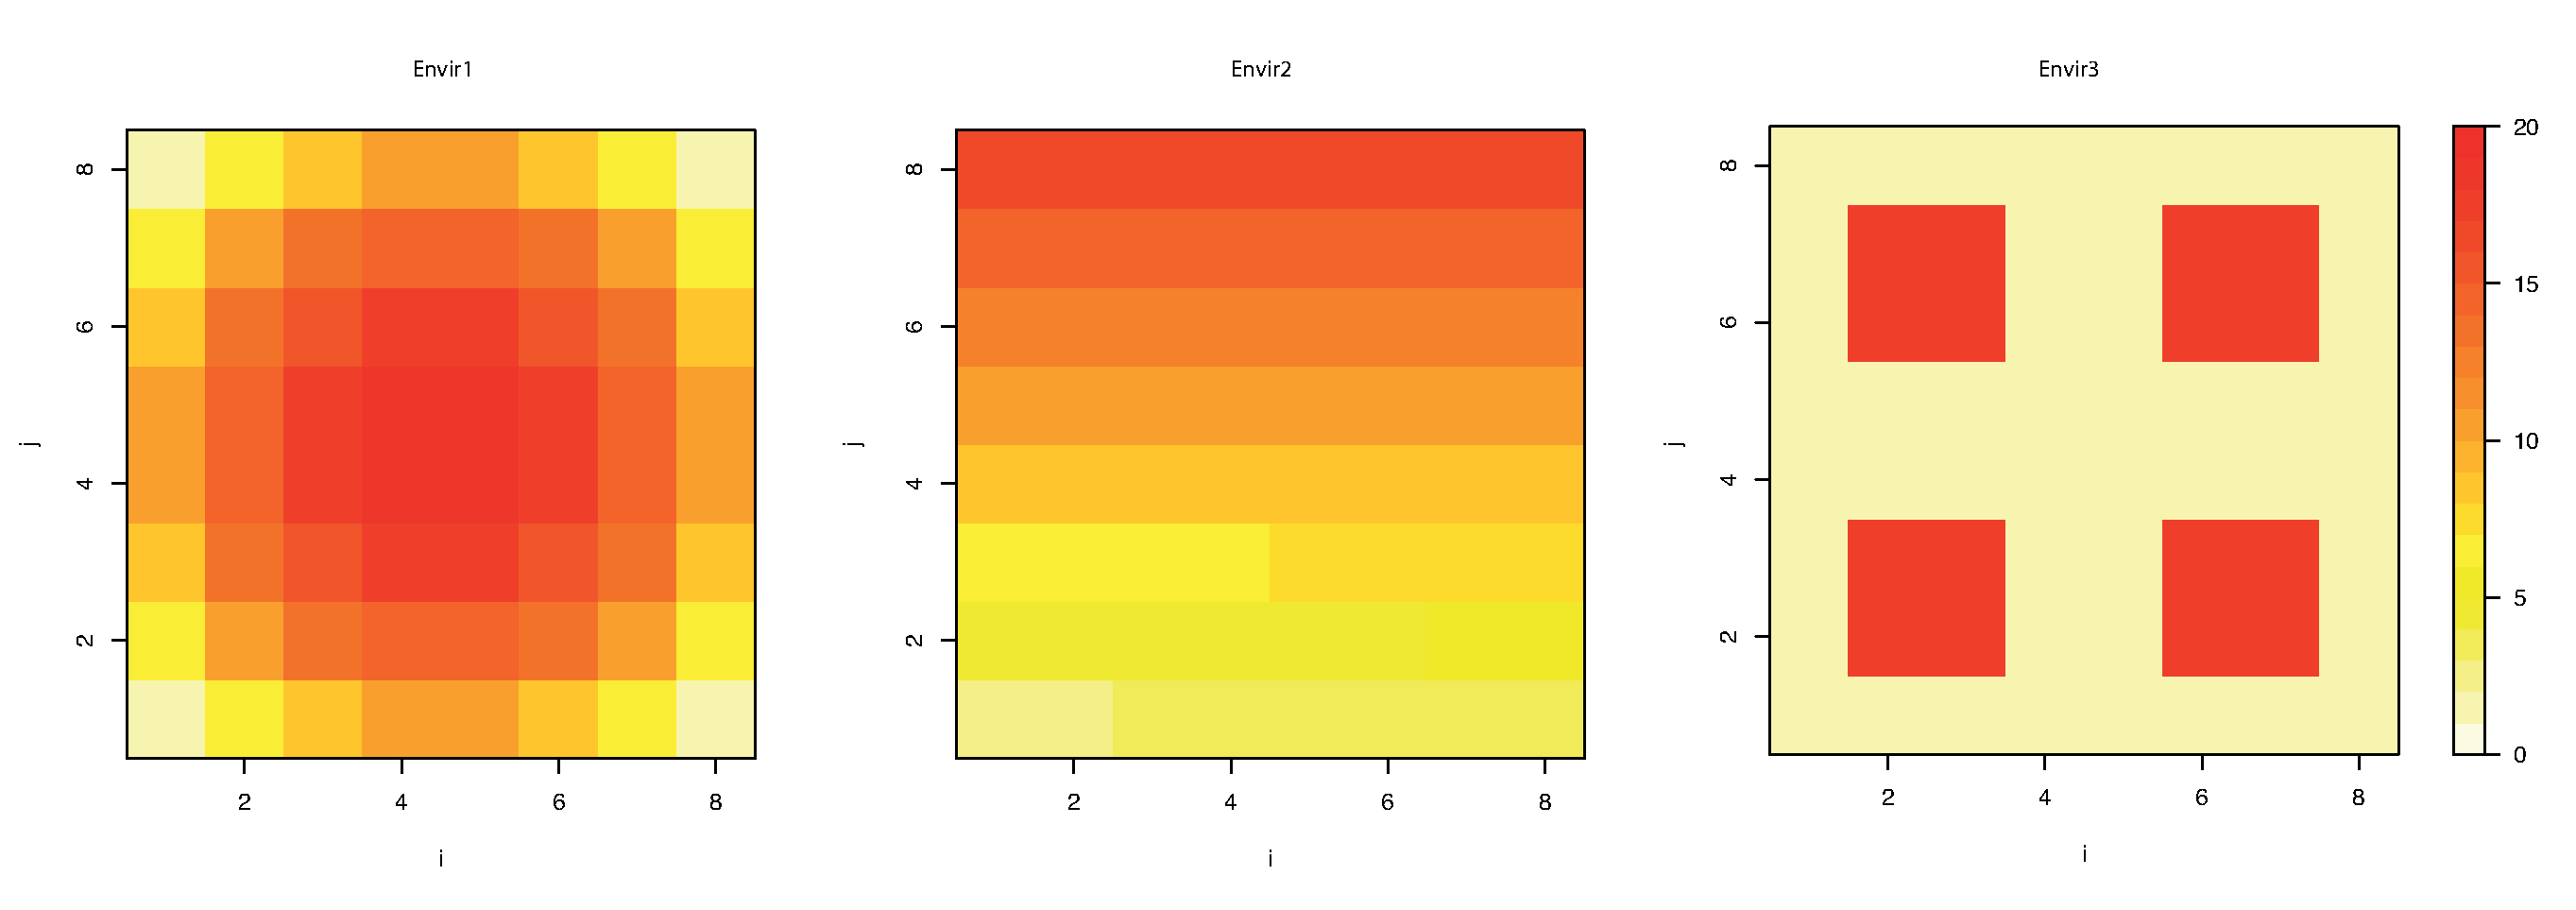
\includegraphics[height=0.25\textheight]{figures/simulatedenvironment.eps}
\end{center}
\caption{Graphical representation of mean environmental value for environment 1, 2 and 3}%
\label{fig:simulatedenvir}%
\end{figure*}



\begin{figure}[t]
\begin{center}
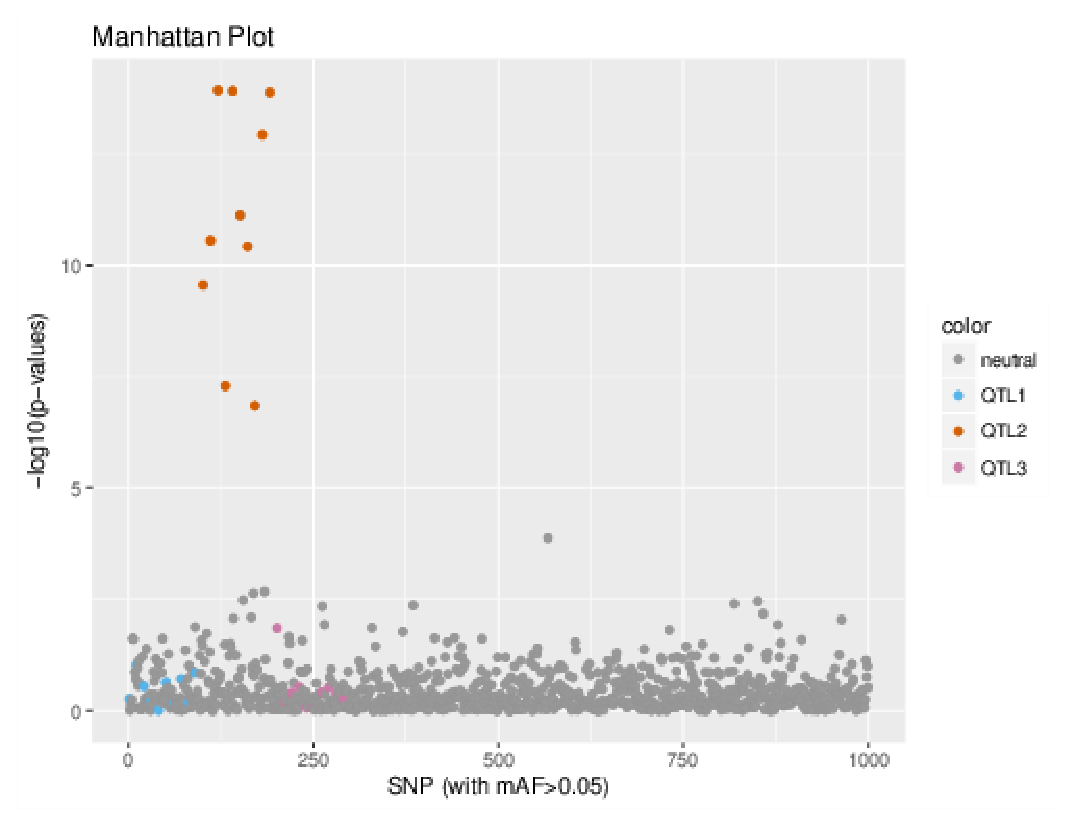
\includegraphics[height=0.21\textheight]{figures/sim5_pcadapt.eps}
\end{center}
\caption{Manhattan plot of the result of pcadapt on a simulated data set.}%
\label{fig:pcadapt}%
\end{figure}

\begin{figure}[t]
\begin{center}
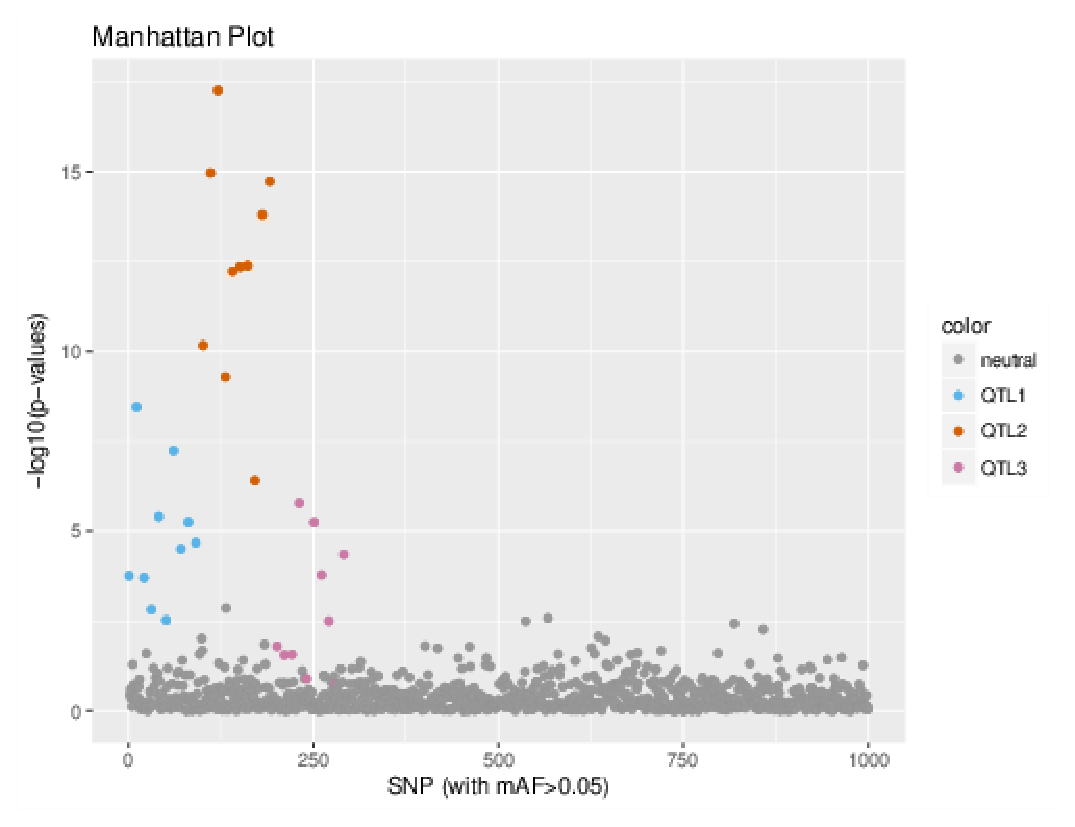
\includegraphics[height=0.21\textheight]{figures/sim5_capscale.eps}
\end{center}
\caption{Manhattan plot of the result of genome scan using RDA on a simulated data set.}%
\label{fig:rda}%
\end{figure}


\begin{figure*}[t]
\begin{center}
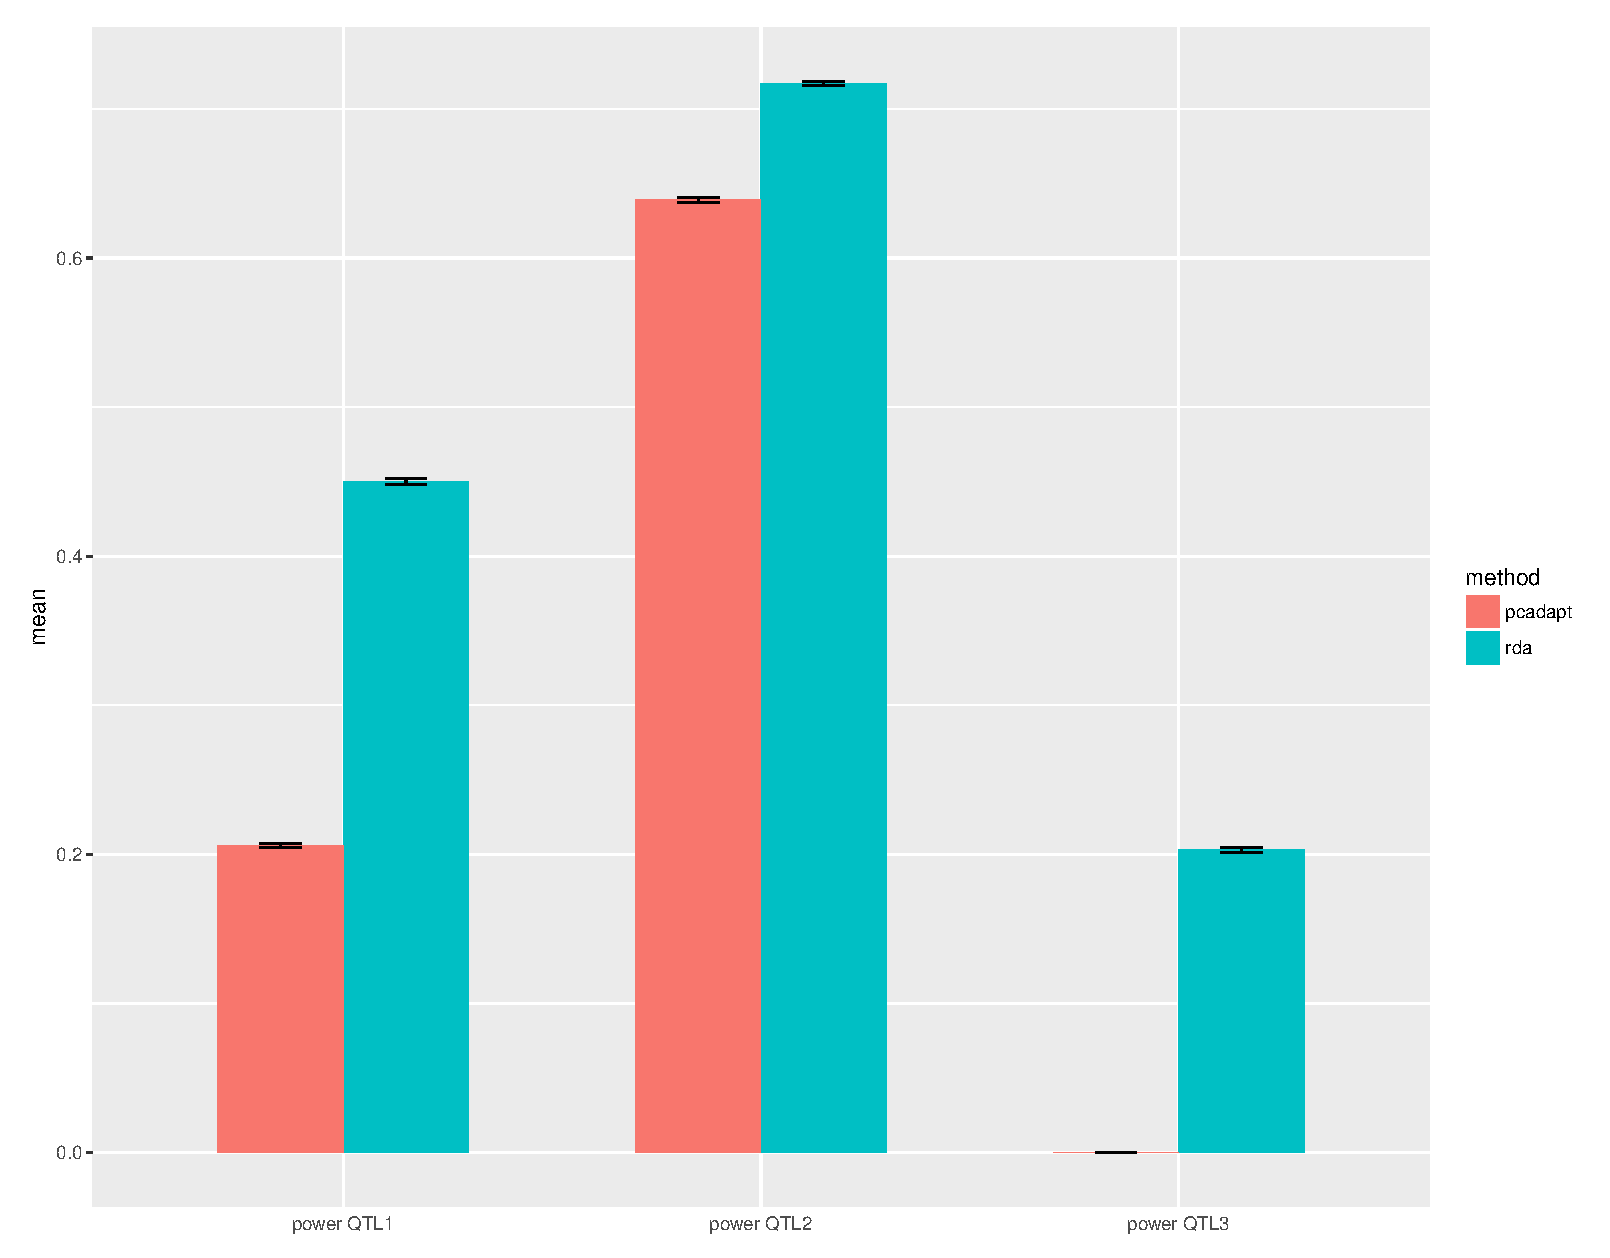
\includegraphics[height=0.4\textheight]{figures/overallresults.eps}
\end{center}
\caption{Performance results of rda and pcadapt methods. Each performance value is averaged over 100 simulated dataset (error bars are displayed but hardly visible since they are very scarce). Power is given seperately for loci coding for quantitative trait 1, 2 and 3.}%
\label{fig:performance}%
\end{figure*}

\subsection{Environmental genomics}

We then performed a second RDA on the "adaptively enriched genetic space" as performed by \citet{Steane2014a} on the same simulated dataset as in Fig. \ref{fig:pcadapt} and \ref{fig:rda} and display its results on Fig. \ref{fig:rdaA}. We did the same analyis and measured the mean $R^2$ between env1, env2 and env3 and each of the first three ordination axis. This is summarized in Fig. \ref{fig:R2}.

\begin{figure*}[t]
\begin{center}
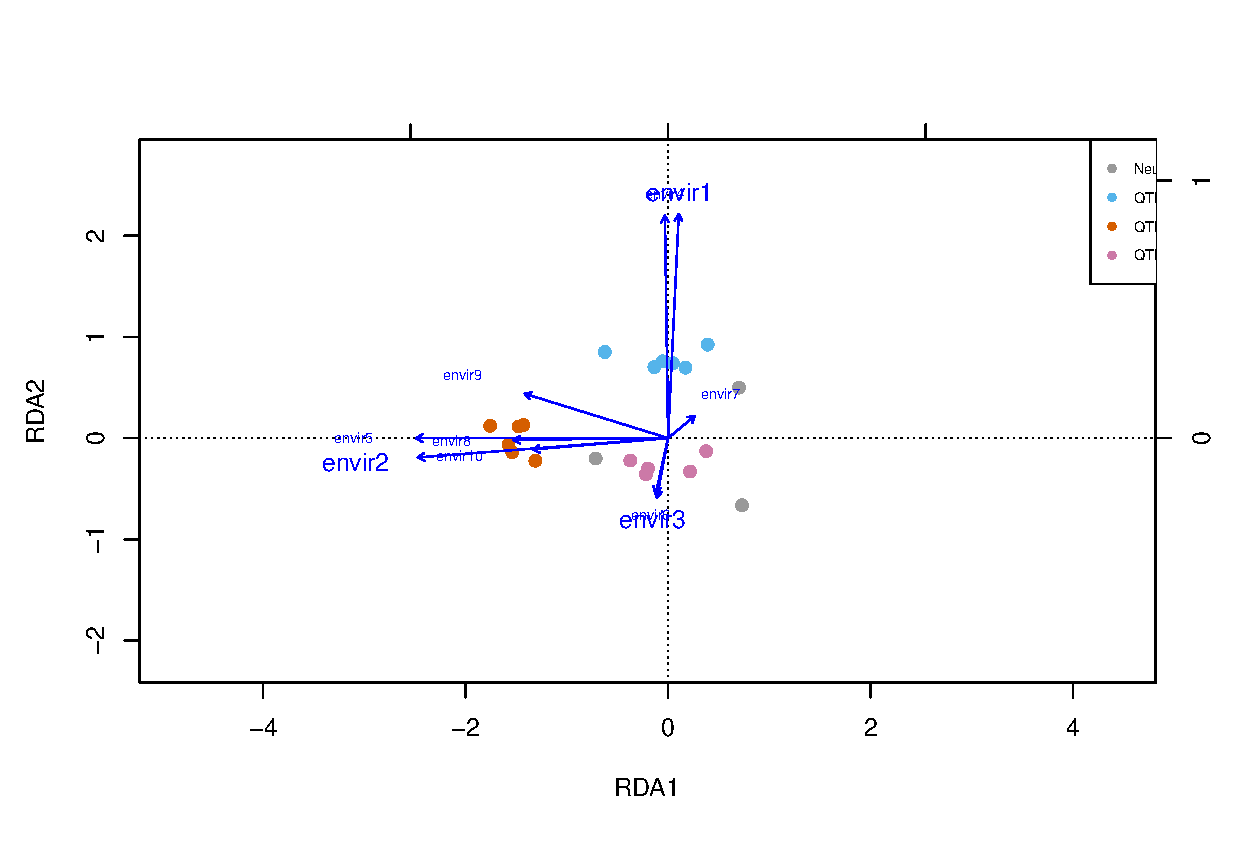
\includegraphics[height=0.4\textheight]{figures/rdaA.eps}
\end{center}
\caption{RDA on the adaptively enriched genetic space. We discarded the individual points for readability. Dots represents outliers SNPs.  $R^2$ of envir1 with the first, second and third axis is (0.02\%, 77.5\%, 14.5\%), envir2 is (99.3\%, 0.003\%, 0001\%) and envir3 is (0.009\%, 0.82\%, 64.7\%)}%
\label{fig:rdaA}%
\end{figure*}

\begin{figure}[t]
\begin{center}
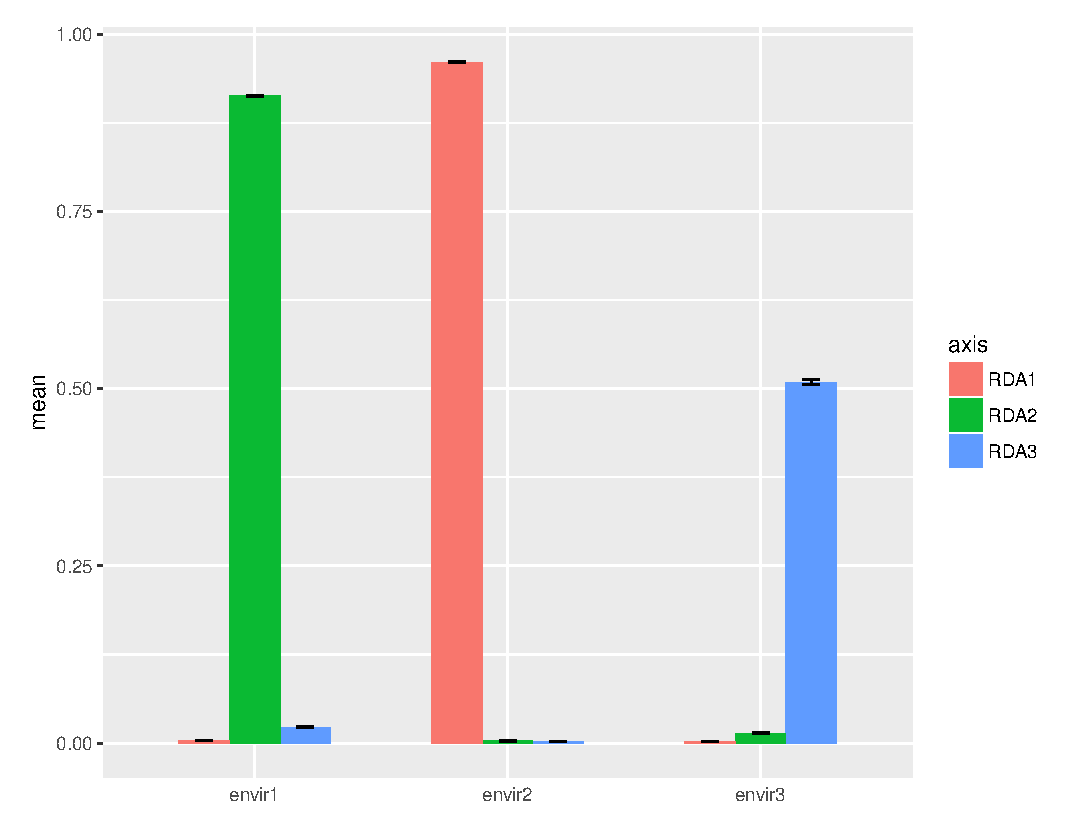
\includegraphics[height=0.21\textheight]{figures/R2.eps}
\end{center}
\caption{$R^2$ between envir1, envir2 and envir3 and each of the first three ordination axis. Values are averaged across the 100 simulated datasets.}%
\label{fig:R2}%
\end{figure}

\subsection{Loblolly Pine}


\section{Discussion}

Fig \ref{fig:pcadapt} shows that pcadapt approach works well when the environmental gradient and the selective pressures are acting in the same direction than the geographical pattern of isolation by distance. Whereas when the environmental gradient is quadratic on the geographical range (QTL1) or when it is a coarse environment (QTL3). Indeed, we can hypothesize that the PCA ordination fails at orienting the genetic space differentiation into the direction of environment 1 and environment 3 therefore leaving no chance to detect any outliers on the QTL influenced by these environmental variables. Fig \ref{fig:rda} shows that RDA has a much better behavior than pcadapt by taking advantage of using informations of environmental local conditions.

Results summarized on Fig \ref{fig:performance} is confirming that both methods have a good control of false discovery rate ($8.36 \times 10^{-2}$ for pcadapt and $8.51 \times 10^{-2}$ for RDA) and that overall RDA shows better performance at detecting true outliers since it succeeds to detect quite often QTL1 and QTL3 SNPs. It seems however less efficient at detecting QTL3 outliers but this might be due to the fact that local adaptation on a coarse environment is more difficult  that adaptation on a smooth environmental gradient as environment 1 and 2. These simulations plead in favor of using constrained ordination method instead of PCA when non genetic data such as environmental variable are available in order to orientate the axis in the direction of informative gradients.

When performing an RDA on the "adaptively enriched genetic space", Fig. \ref{rdaA} and \ref{R2} show that the method succeed at detecting the relevant selective gradient and separating them on different axis at least on our simulations. This therefore serves as a proof of concept of \citet{Steane2014a}'s approach to represent multilocus selective gradient and the possibility to use the ordination axis it to devise a metric that provides a holistic measure of genomic adaptation. Indeed, in RDA1 is strongly associated with envir2, RDA2 with envir1 and RDA3 with envir3 whereas poorly associated with the other axis. As expected, the correlated environment are also strongly associated with this respective axis. This is reflecting the fact that in reality it is difficult on an environmental gradient to distinguish  among the covariable which one has a causal effect on the individual fitness. However, it is often sufficient for biologists when performing an exploratory analysis to identify combination of environment variable having a strong association with adaptive variation without knowing precisely the underlying mechanical process.


\section{Supplementary Material}


\section{Acknowledgments}



\bibliographystyle{natbib}%%%%natbib.sty
\bibliography{Article_ca_gs}%%%refs.bib

\end{document}